\documentclass{lehramt-informatik-aufgabe}
\liLadePakete{er,syntax}
\begin{document}

\section{Aufgabe 5: ER-Diagramm und Relationenmodell vertieft
\index{Entity-Relation-Modell}
\footcite[Thema 1 Teilaufgabe 2 Aufgabe 1]{examen:46116:2013:03}}

Sie sollen ein System zur Verwaltung von Pferderennen entwerfen.
Gehen Sie dabei von folgendem Szenario aus:
\footcite{db:pu:1}

\begin{itemize}
\item \mpEntity{Unternehmen} werden ihre eindeutige
\mpAttribute{Unternehmens-ID} identifiziert. Sie haben eine
\mpAttribute{Adresse} und \mpRelationship{besitzen} Rennställe.

\item Der \mpAttribute{Name} eines \mpEntity{Rennstalls} ist nur
innerhalb eines Unternehmens eindeutig. Für jeden Rennstall wird das
\mpAttribute{Gründungsdatum} gespeichert.

\item \mpEntity{Pferde} \mpRelationship{gehören} immer zu einem
Rennstall. \mpAttribute{Pferdenamen} werden in einem Rennstall nur
jeweils maximal einmal vergeben.

\item \mpEntity{Jockeys} sind in einem Rennstall
\mpRelationship{beschäftigt}. Jeder Rennstall vergibt seine eigenen
\mpAttribute{Personalnummern}. Für jeden Jockey werden
\mpAttribute{Vorname} und \mpAttribute{Name} gespeichert.

\item \mpEntity{Rennen} haben ein \mpAttribute{Datum}, ein
\mpAttribute{Preisgeld} und einen \mpAttribute{Namen}, über den sie
identifiziert werden.

\item Unternehmen \mpRelationship{unterstützen} Rennen finanziell mit
einem bestimmten Betrag.

\item Jockeys \mpRelationship{nehmen} mit Pferden an Rennen teil. Im
Rennen erreichen sie einen bestimmten Platz. Die Kombination aus Jockey
und Pferd ist nicht fest, bei unterschiedlichen Rennen können Jockeys
verschiedene Pferde reiten. Jockeys können auch mit Rennpferden von
fremden Rennställen, die anderen Unternehmen gehören können, an Rennen
teilnehmen.
\end{itemize}

\begin{enumerate}

%%
% (a)
%%

\item Entwerfen Sie für das beschriebene Szenario ein
ER-Modell. Bestimmen Sie hierzu:

\begin{itemize}
\item die Entity-Typen, die Relationship-Typen und jeweils deren
Attribute,

\item ein passendes ER-Diagramm,

\item die Primärschlüssel der Entity-Typen, welche Sie anschließend in
das ER-Diagramm eintragen, und

\item die Funktionalitäten der Relationship-Typen, welche Sie ebenfalls
in das ER-Diagramm eintragen.
\end{itemize}

%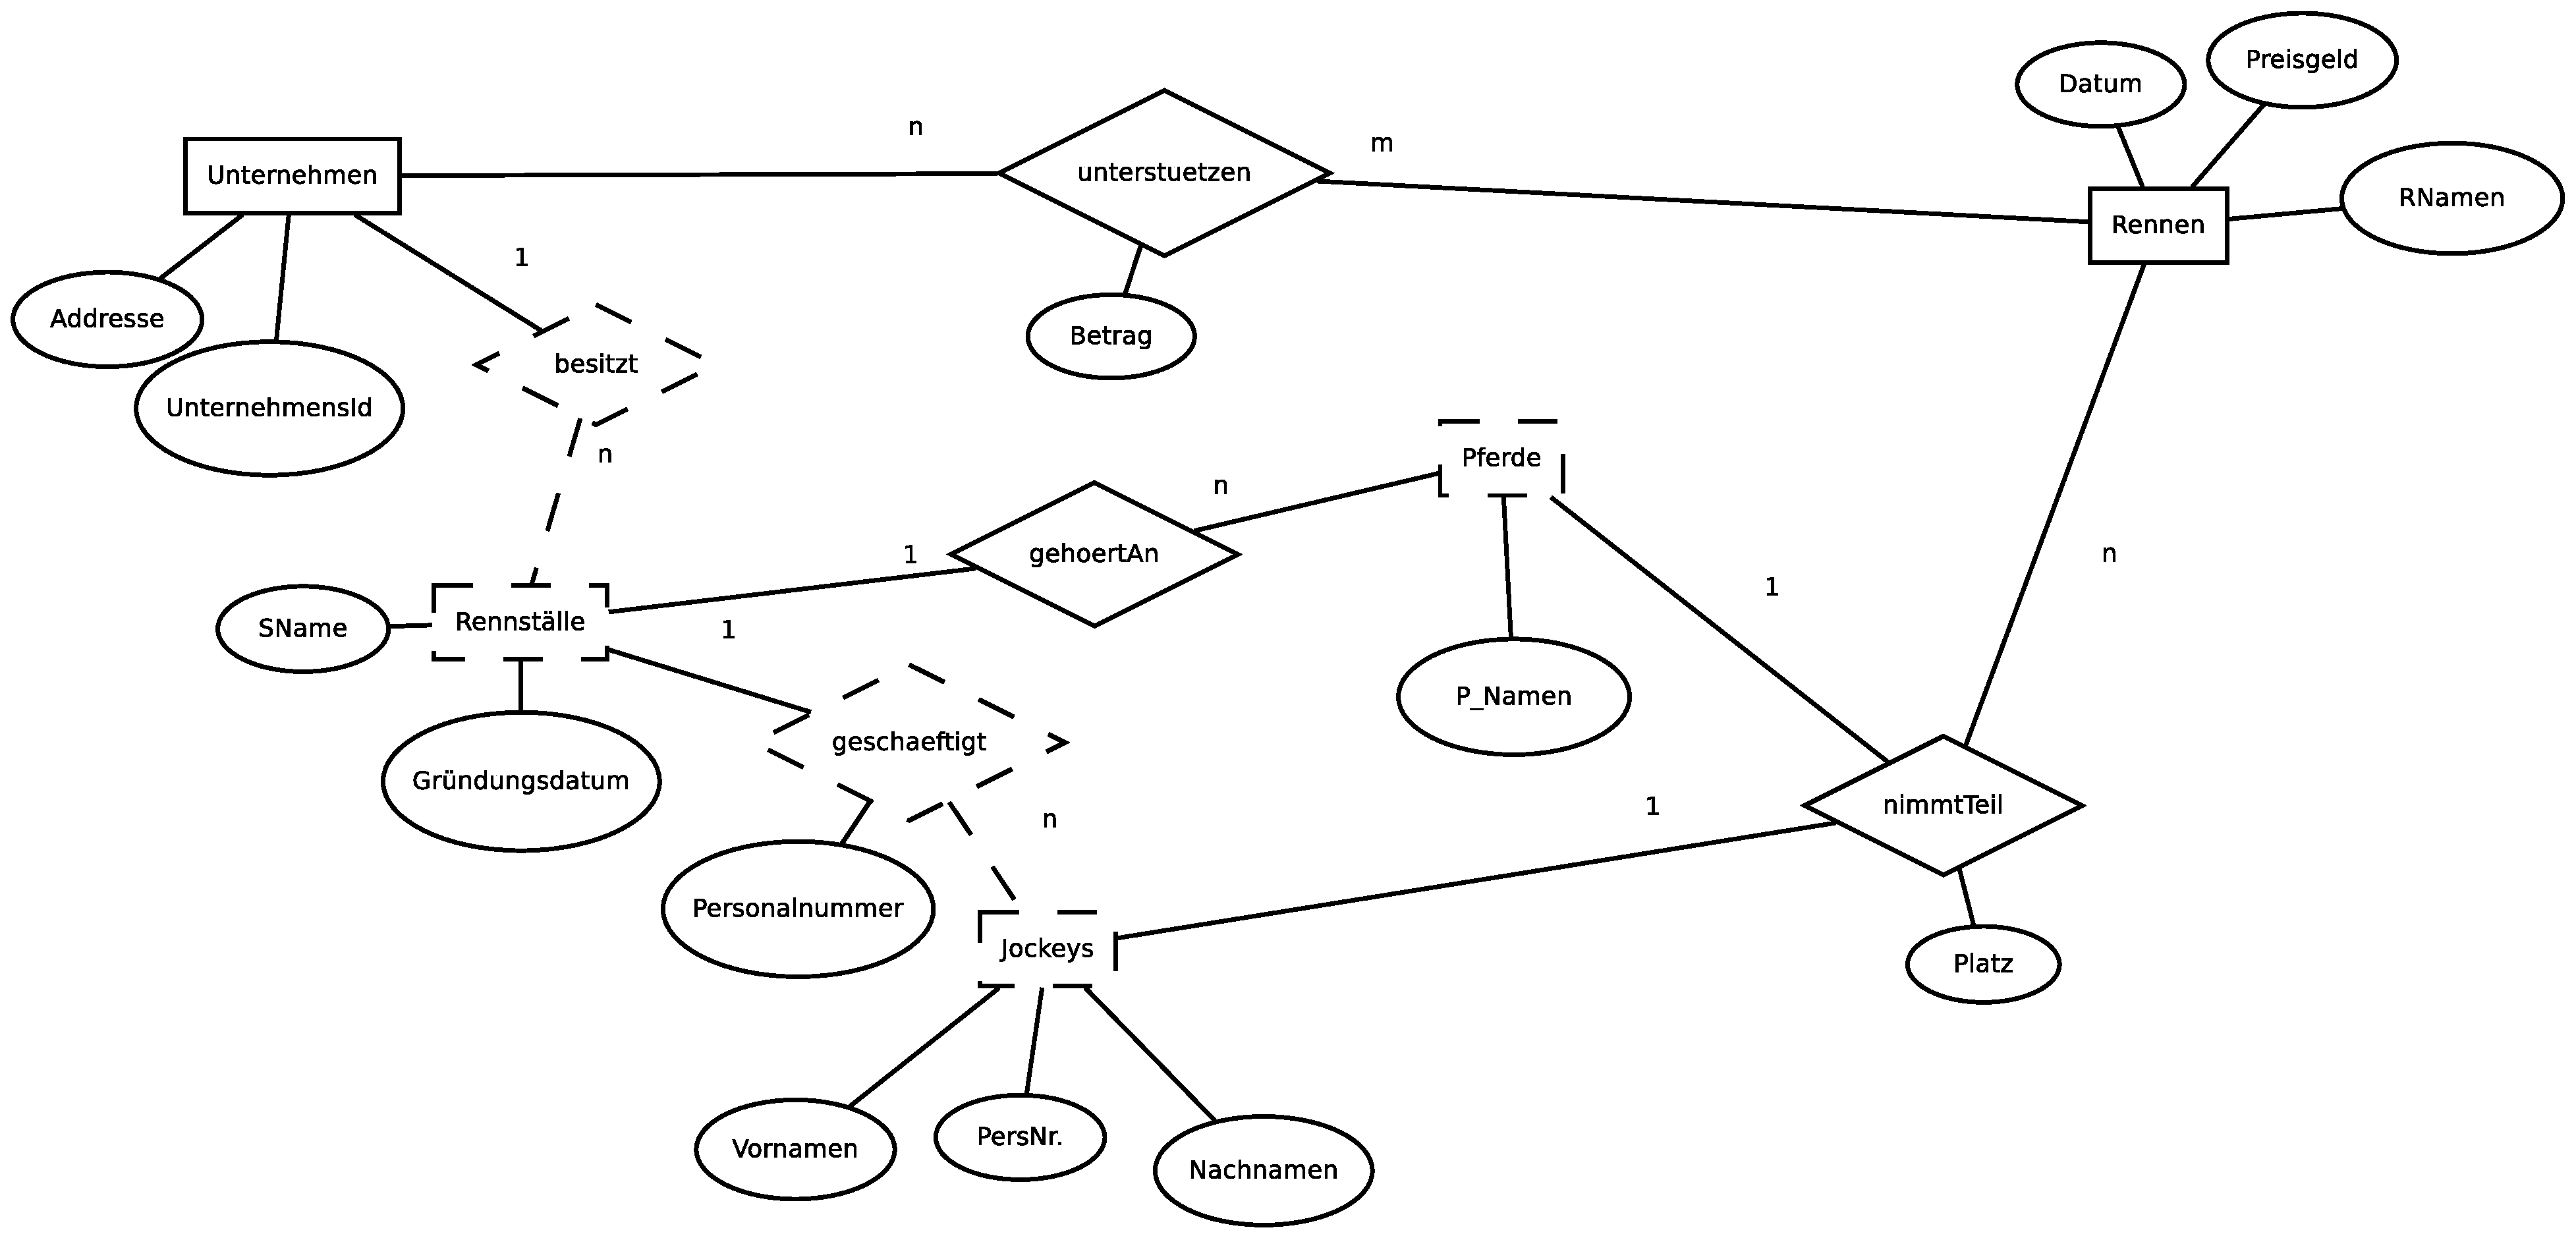
\includegraphics[width=\linewidth]{Rennstaelle.eps}

\begin{antwort}
\begin{center}
\begin{tikzpicture}[er2,scale=0.6,transform shape]
% Unternehmen
\node[entity] (Unternehmen) {Unternehmen};
\node[attribute,above=0.5cm of Unternehmen] (UID) {\key{UID}} edge (Unternehmen);
\node[attribute,left=0.5cm of Unternehmen] (Adresse) {Adresse} edge (Unternehmen);

% Rennstall
\node[weak entity,right=5cm of Unternehmen] (Rennstall) {Rennstall};
\node[attribute,above=0.5cm of Rennstall] (Name) {Name} edge (Rennstall);
\node[attribute,right=0.5cm of Rennstall] (Gründungsdatum) {Gründungsdatum} edge (Rennstall);

% besitzt
\node[ident relationship,right=1.5cm of Unternehmen] (besitzt) {besitzt}
  edge node[auto]{1} (Unternehmen)
  edge[weak] node[auto]{n} (Rennstall);

% Pferd
\node[weak entity,below=4cm of Rennstall] (Pferd) {Pferd};
\node[attribute,right=0.5cm of Pferd] (Name) {\key{Pferdename}}
  edge (Pferd);

% gehören
\node[ident relationship,below=1.5cm of Rennstall] (gehören) {gehören}
  edge node[auto]{1} (Rennstall)
  edge[weak] node[auto]{n} (Pferd);

% Jockey
\node[weak entity,below=4cm of Unternehmen] (Jockey) {Jockey};
\node[attribute,left=0.5cm of Jockey] (Personalnummer) {\key{Personalnummer}}
  edge (Jockey);
\node[attribute,below left=0.5cm of Jockey] (Vorname) {Vorname}
  edge (Jockey);
\node[attribute,below=0.5cm of Jockey] (Name) {Name}
  edge (Jockey);

% beschäftigt
\node[relationship,below=1cm of Unternehmen] (beschäftigt) {beschäftigt}
  edge node[auto]{1} (Unternehmen)
  edge node[auto]{n} (Jockey);

% Rennen
\node[entity,below right=2cm of Jockey] (Rennen) {Rennen};
\node[attribute,below left=0.5cm of Rennen] (Datum) {Datum}
  edge (Rennen);
\node[attribute,below=0.5cm of Rennen] (Preisgeld) {Preisgeld}
  edge (Rennen);
\node[attribute,below right=0.5cm of Rennen] (Name) {Name}
  edge (Rennen);

\node[relationship,right=1cm of Jockey] (teilnehmen) {teilnehmen}
  edge node[auto]{1} (Jockey)
  edge node[auto]{1} (Pferd)
  edge node[auto]{n} (Rennen);
\end{tikzpicture}
\end{center}
\end{antwort}

%%
% (b)
%%

\item Überführen Sie das ER-Modell aus Aufgabe a) in ein verfeinertes
relationales Modell. Geben Sie hierfür die verallgemeinerten
Relationenschemata an. Achten Sie dabei insbesondere darauf, dass die
Relationenschemata keine redundanten Attribute
enthalten.\index{Relationenmodell}

\begin{minted}{md}
Unternehmen (UnternehmensID, Addresse)
Rennstall (S_Name, UnternehmensID[Unternehmen], Gründungsdatum)
Jockey (PersNr, S_Name[Rennstall], ID[Unternehmen], Vorname, Name)
Rennen (R_Name, Datum, Preisgeld)
Pferd (P_Name, S_Namen, UnternehmensID[Unternehmen])

teilnehmen (R_Name[Rennen], PersNr[Jockey], S_Name1, ID1, P_Namen, S_Namen2, ID2, Platz)
unterstuetzen (UnternehmensID[Unternehmen], R_Name[Rennen], Betrag)
\end{minted}
\end{enumerate}
\end{document}
